\documentclass[a4paper, 11pt]{article}
\usepackage{comment}  
\usepackage{fullpage} 
\usepackage[hidelinks]{hyperref}
\usepackage{amsmath}
\usepackage{graphicx}

\usepackage{booktabs} 

\usepackage[ruled]{algorithm2e} 
\renewcommand{\algorithmcfname}{ALGORITHM}

\begin{document}

\noindent
\large\textbf{PROBLEM 4.} \hfill \textbf{Dhruviben Modi} \\
\normalsize SOEN 6011 \hfill \textbf{40166396} \\
 SOFTWARE ENGINEERING PROCESSES \hfill Due Date: August 5, 2022 \\
\hfill Github address : git@github.com:mdhruvi/SOEN-6011-project.git


\section{Error Handling and Messaging}
\indent\indent Maintaining the application's regular flow is the major benefit of exception handling. Exception is an unwanted or unexpected event, which occurs during the execution of a program\\

In Gamma Function calculator, if user enters any invalid input ($n = 0, n < 0, n > 171$), then the program will notify user with an error message containing "Infinity" as Gamma value of such numbers are positive infinity\\

Additionally, when a user accidentally enters a String, then in such case program throws an InputmisMatchException with a message that "Please enter correct input". In Gamma Function, exceptions are handled using try..catch method.\\

\section{Quality Attributes}
\begin{itemize}
    \item{Usability : To calculate the corresponding value of $\Gamma \left( n \right)$, the user only needs to enter the value of $n$, if the input is correct then the system returns the calculated value otherwise for the invalid input, the system also returns the exception that the input is not valid, which can help the user to easily perform the gamma function.}
    
    \item{Robustness : System can take positive real numbers, if the input is not valid then the system simply throws an exception and prints the error handling message containing "Invalid input", but the system will not crash. }
    
    \item{Efficient : The system is effective, which is made possible by a straightforward and uncomplicated method; As a result, the user will receive a prompt response within a second of entering correct input, whereas the system prints "Infinity" promptly when user enters $0$, less than $0$ and greater than $171$ as input. }
    
    \item{Maintainability : The separation of the function modules makes the system maintainable. The project's code follows standard programming practises, and each function and variable has a name that makes it clear what it does. Javadoc is written for each function hence the workload for maintenance is minimal.}
    
    \item{Correctness : The system's main requirement is correctness and precision. By using Stirling's formula for valid input, the application process will provide a reasonably accurate output.}
\end{itemize}

\newpage

\section{Debugger}
Finding and resolving errors in a program's source code is the process of debugging. Debugging tools are offered by contemporary IDEs like Eclipse, making it simpler for developers to interactively go through their code and analyse it to find and fix any flaws. To assist a developer in debugging successfully and efficiently, the Eclipse Java IDE offers a variety of debugging tools and perspectives grouped in the Debug Perspective.
\subsection{Advantages}
\begin{itemize}
    
    \item{It is efficient, does not require coding knowledge, and provides the greatest context for identifying issues.}
    
    \item{Error happens in a specific function, but code does not use that function until after the programme has been running for a while. Breakpoints specify where to "pause" a program's execution for the debugger. This makes it possible for you to access the desired area of the software fast.}
    
    \item{One of a debugger's most potent capabilities is single-stepping, which enables a reverse engineer to carry out a single instruction at a time before handing back control to the debugger.}
\end{itemize}

\subsection{Disadvantages}
\begin{itemize}
    \item{It requires human engagement, has a fair learning curve, is not always accessible, and cannot persist output.}
    
    \item{Another drawback of debugger is that the programmer cannot select which method to enter when there are several method calls because it lacks the wise step into function.}
\end{itemize}

\begin{figure}[h]
    \centering
    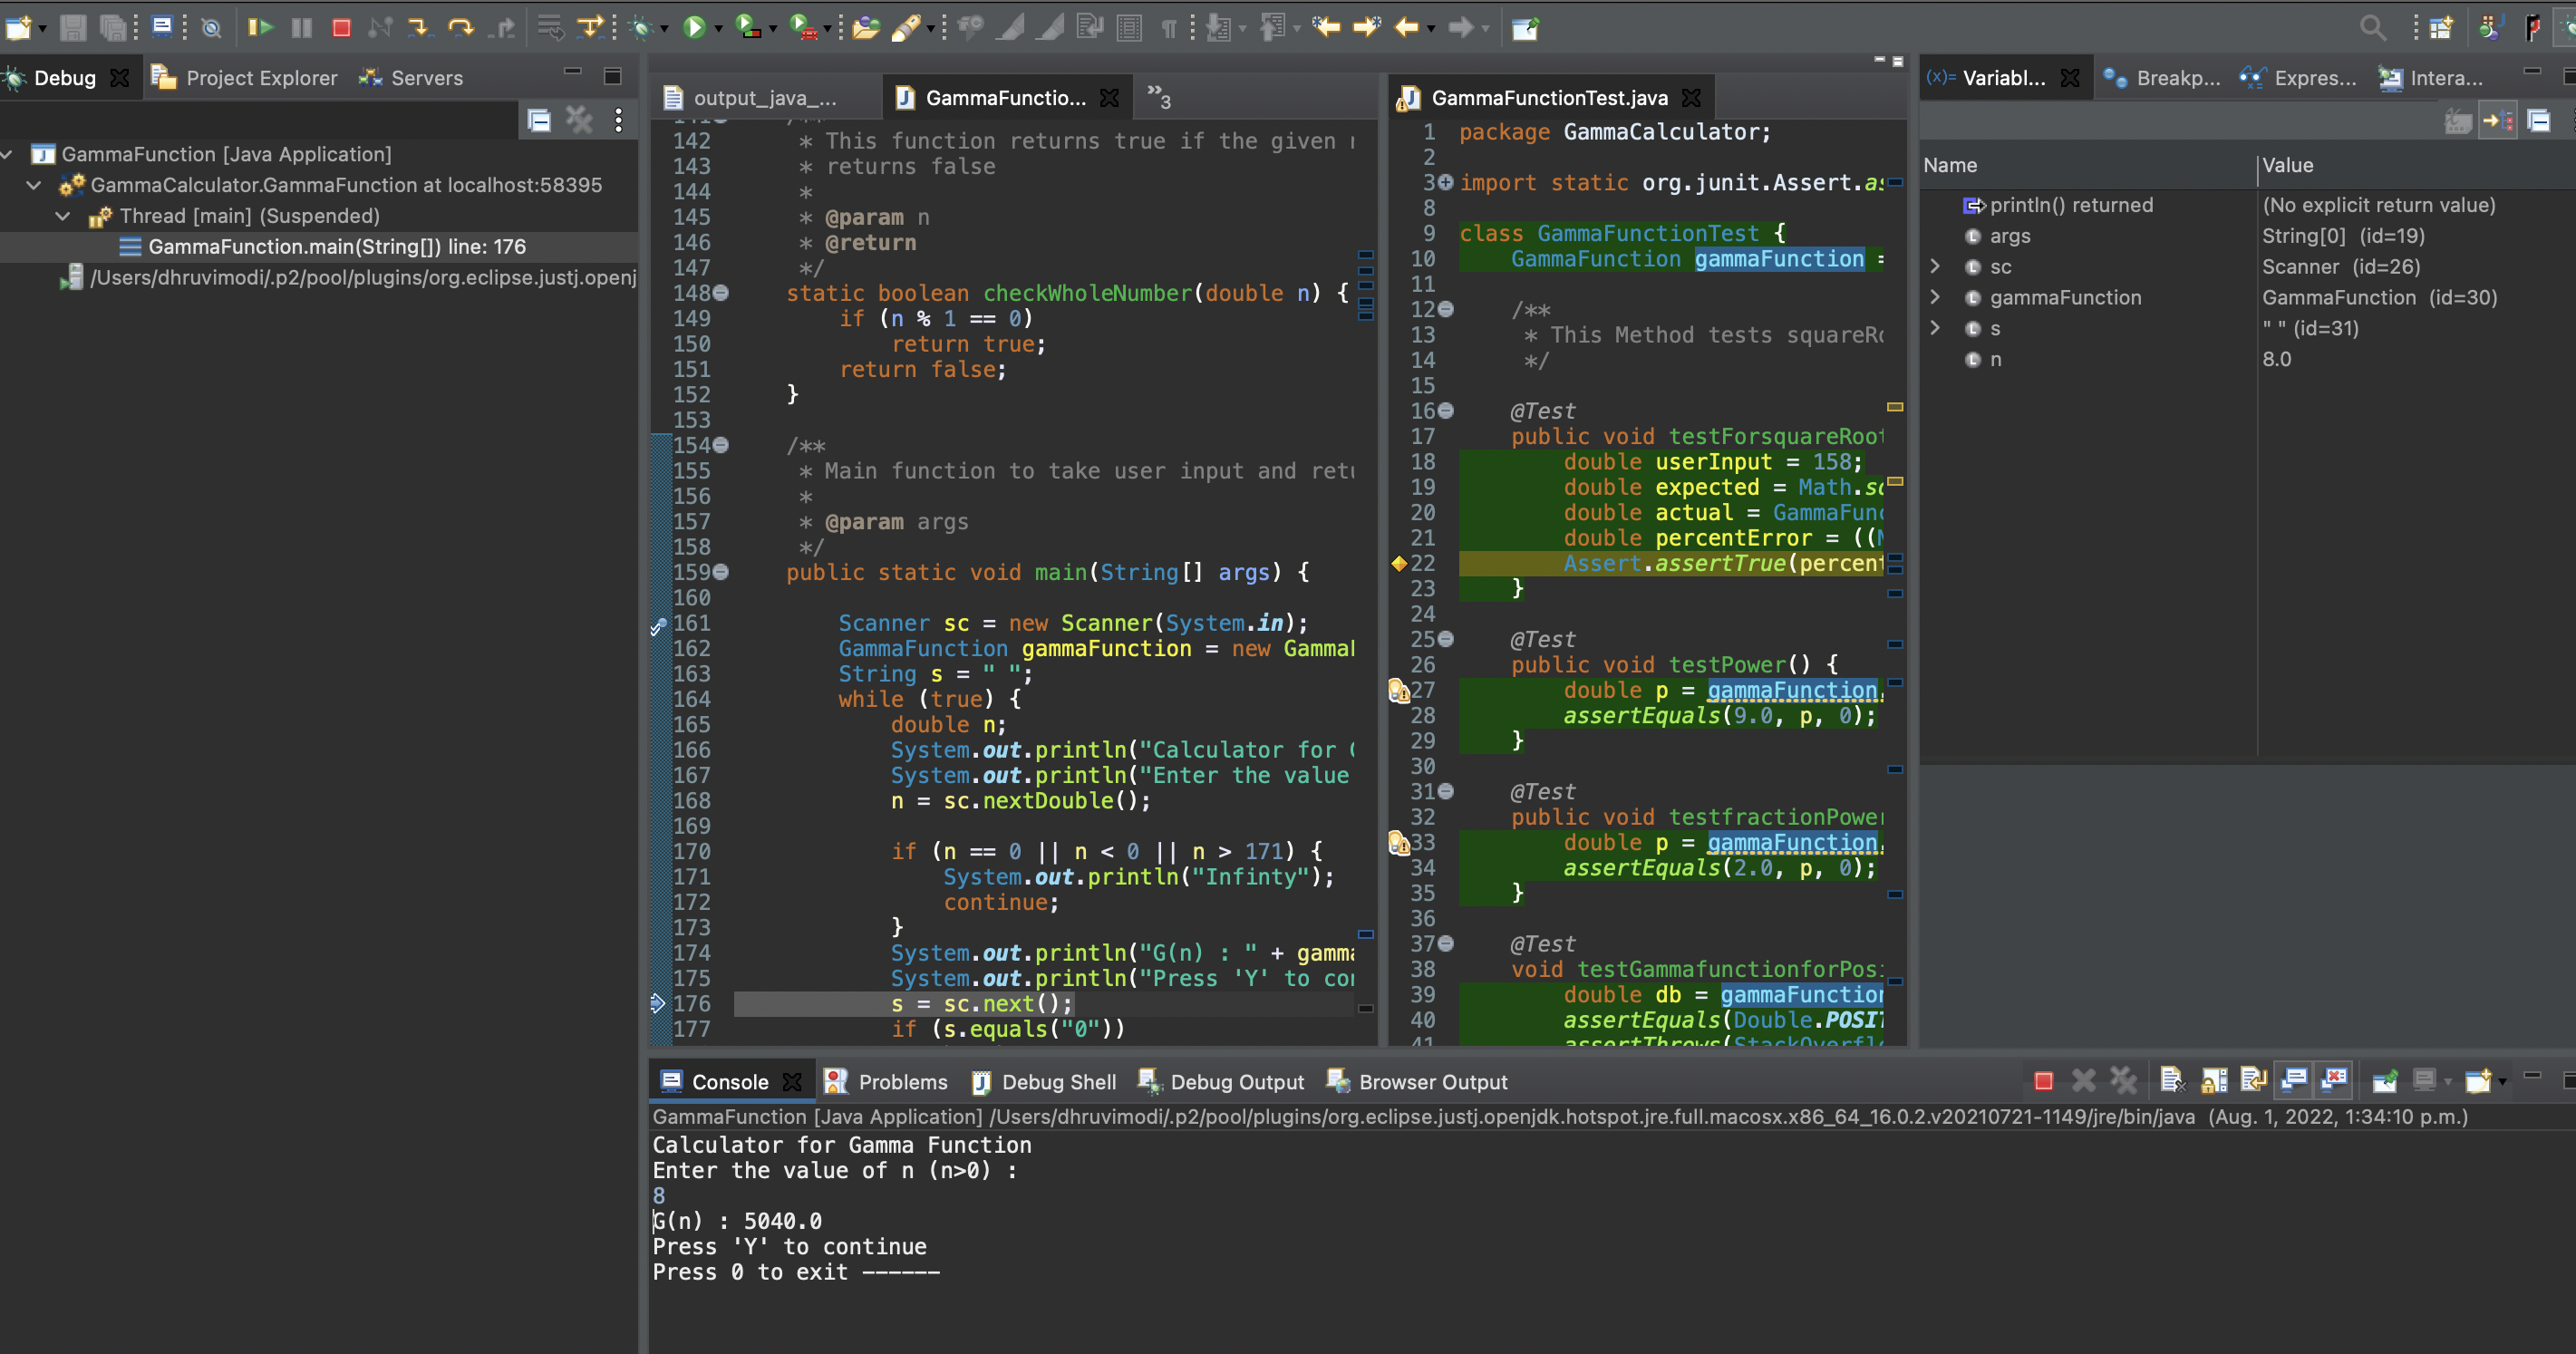
\includegraphics[width=0.9\linewidth]{Images/Debugger.jpg}
    \caption{Screenshot of debugging of Gamma Function.}
    \label{fig:Debugger}
\end{figure}

\section{Tool-Checkstyle}
Java developers can use the Open Source development tool Checkstyle to make sure their code complies with a set of coding standards. The static source code analyzer Checkstyle is integrated into the Eclipse IDE by the Eclipse Checkstyle Plugin (eclipse-cs).

\subsection{Advantages}
\begin{itemize}
    \item{Due to the fact that checkstyle was initially intended to be an independent framework, it is much simpler to combine it with other technologies.}
    
    \item{Code specification verification can be automated with CheckStyle, the key components of the checking include Javadoc comments, name conventions, titles, line lengths, the use of imports and scope modifiers, intervals between characters, etc.}
    
    \item{Team projects benefit from improved code readability, higher project quality, and simpler project maintenance.}
    
    \item{It has the expertise its own rules for developers. Although checkstyle includes more styles than Eclipse does and allows programmers to create their own unique rules,}
\end{itemize}

\subsection{Disadvantages}
\begin{itemize}
    \item{Javac must be able to compile the code in order to find legitimate violations. If not, parsing errors are challenging to comprehend.}
    
    \item{It is difficult to ascertain the type of an expression and its whole inheritance structure.}
    
    \item{The binary Byte Order Mark (BOM) of a file cannot be handled effectively by Checkstyle. In addition, each file is processed separately, making it impossible to view the contents of other files while doing checks.}
\end{itemize}

\begin{figure}[h]
    \centering
    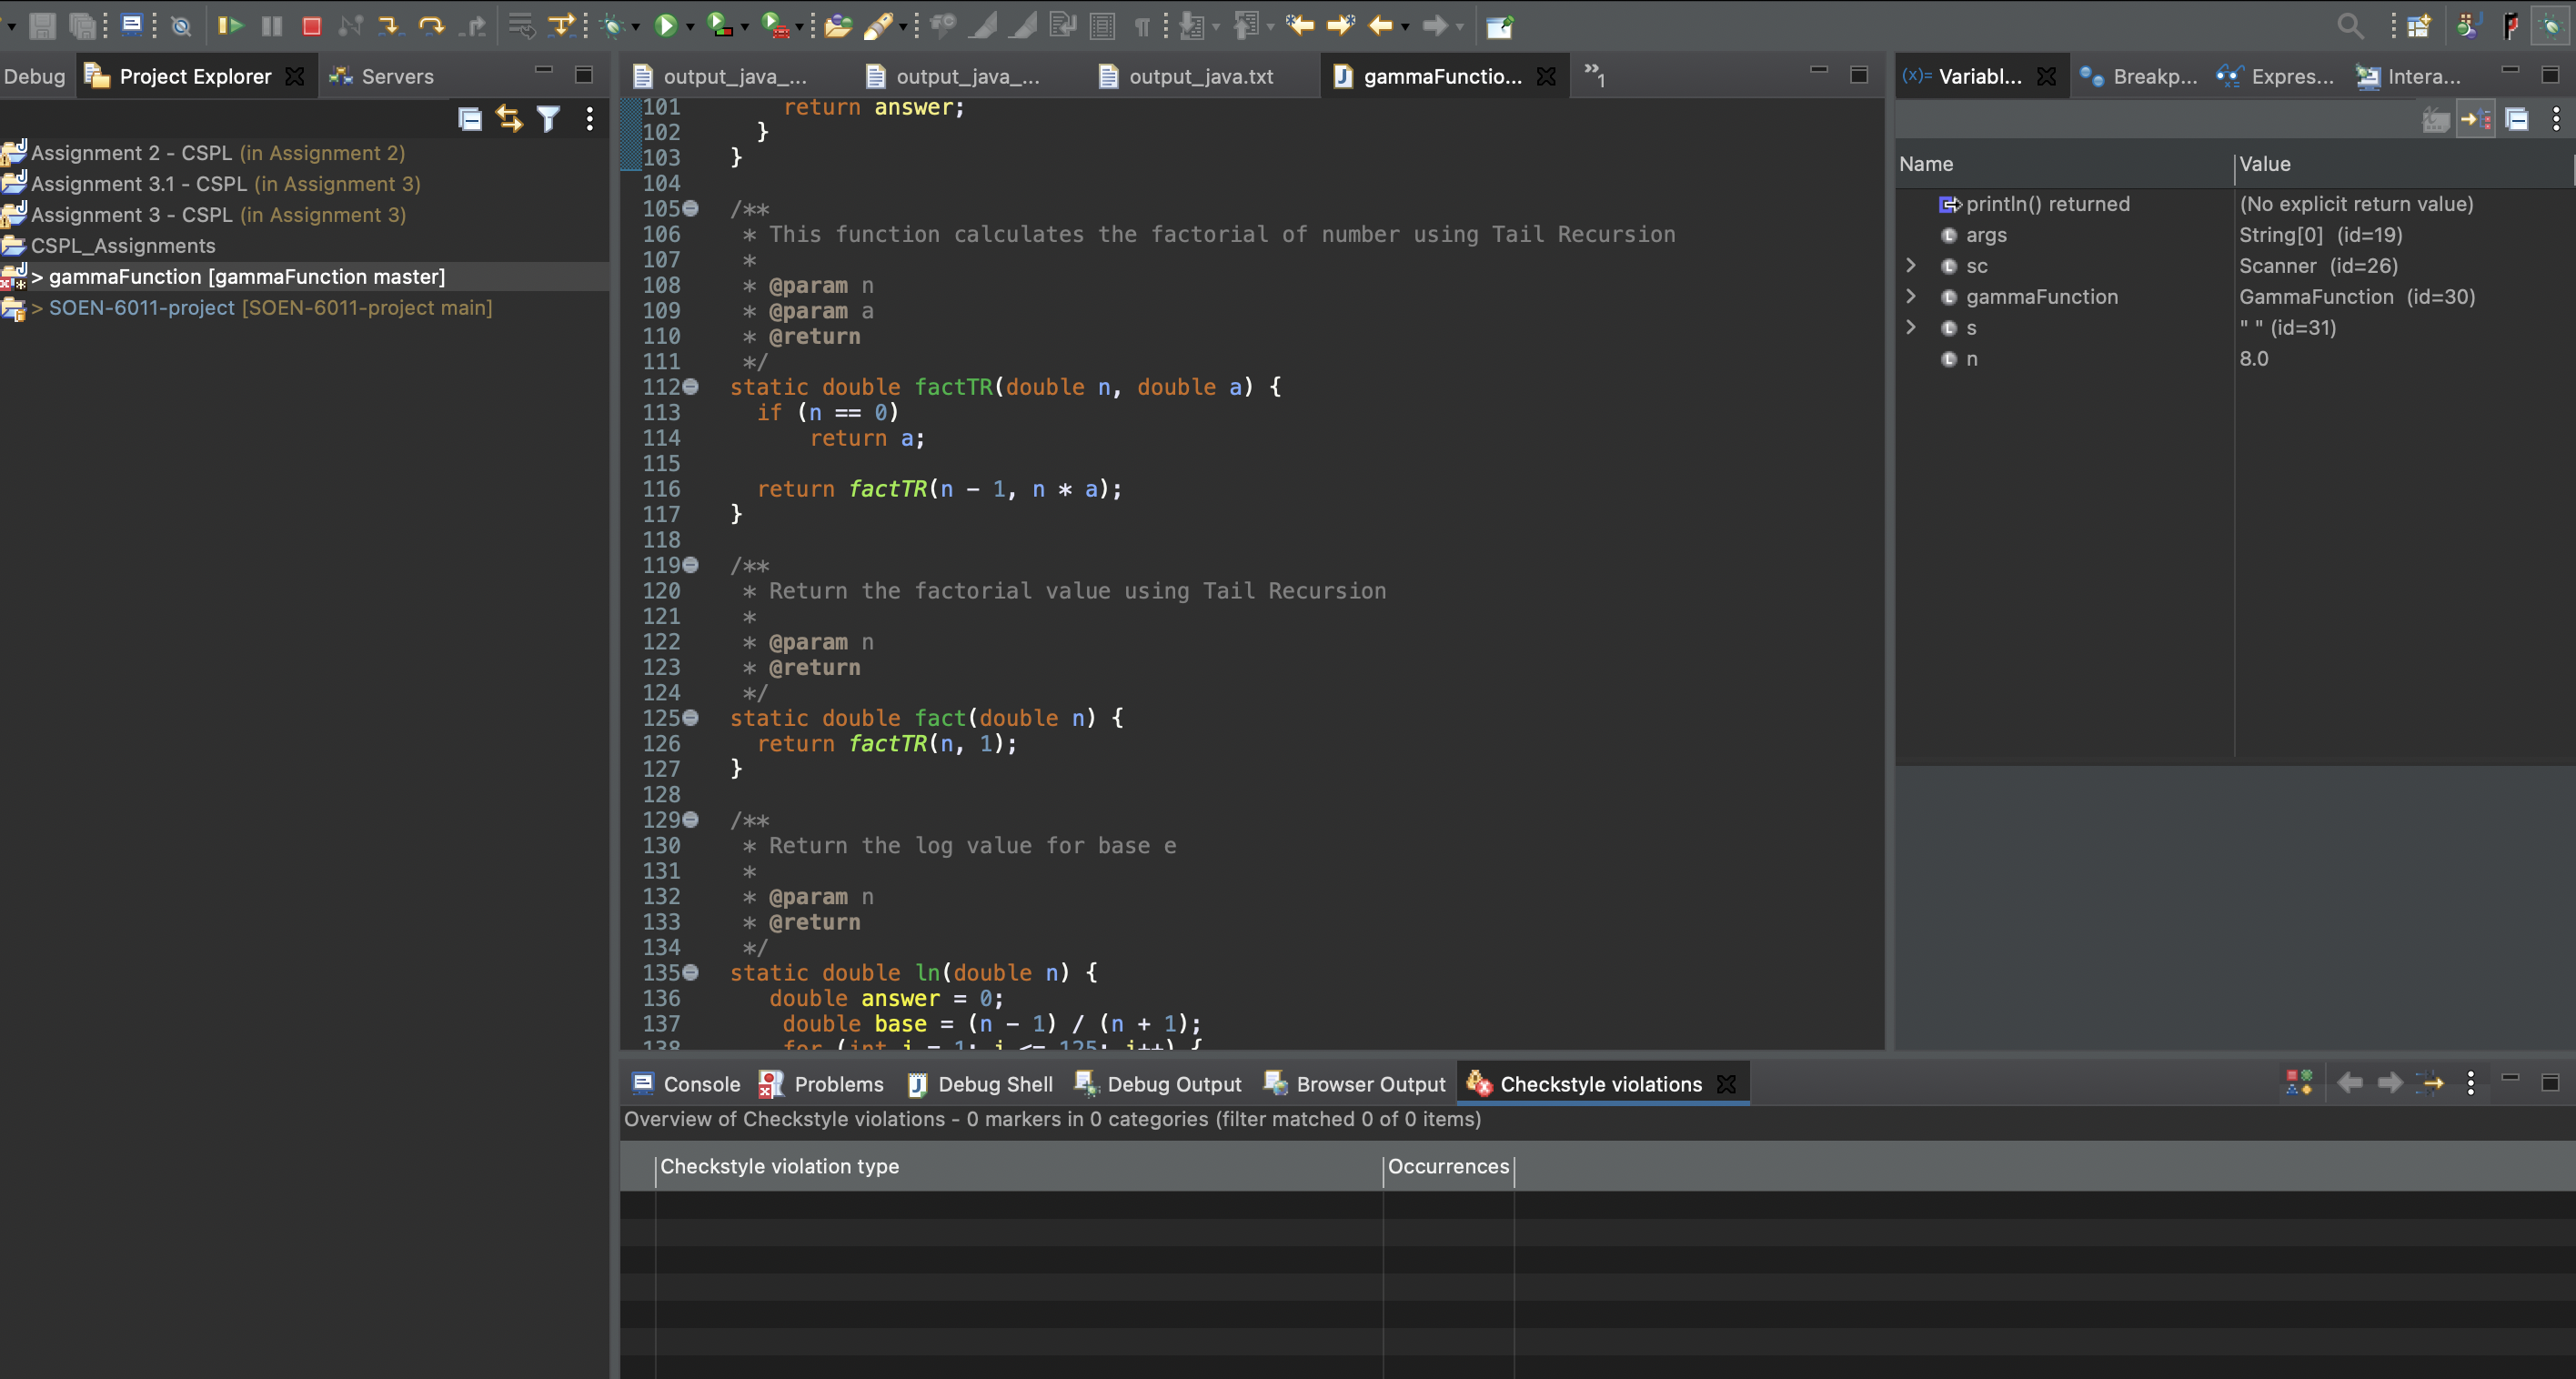
\includegraphics[width=0.9\linewidth]{Images/Typechecking.jpg}
    \caption{Screenshot of Checkstyle of Gamma Function.}
    \label{fig: Checkstyle tool}
\end{figure}

\newpage

\section{PMD}
PMD is a very adaptable tool, this tool analyses source code. It detects typical programming errors such as unneeded variables, empty catch blocks, pointless object creation, etc. CPD, or the copy-paste detector, is included.\\

\begin{figure}[h]
    \centering
    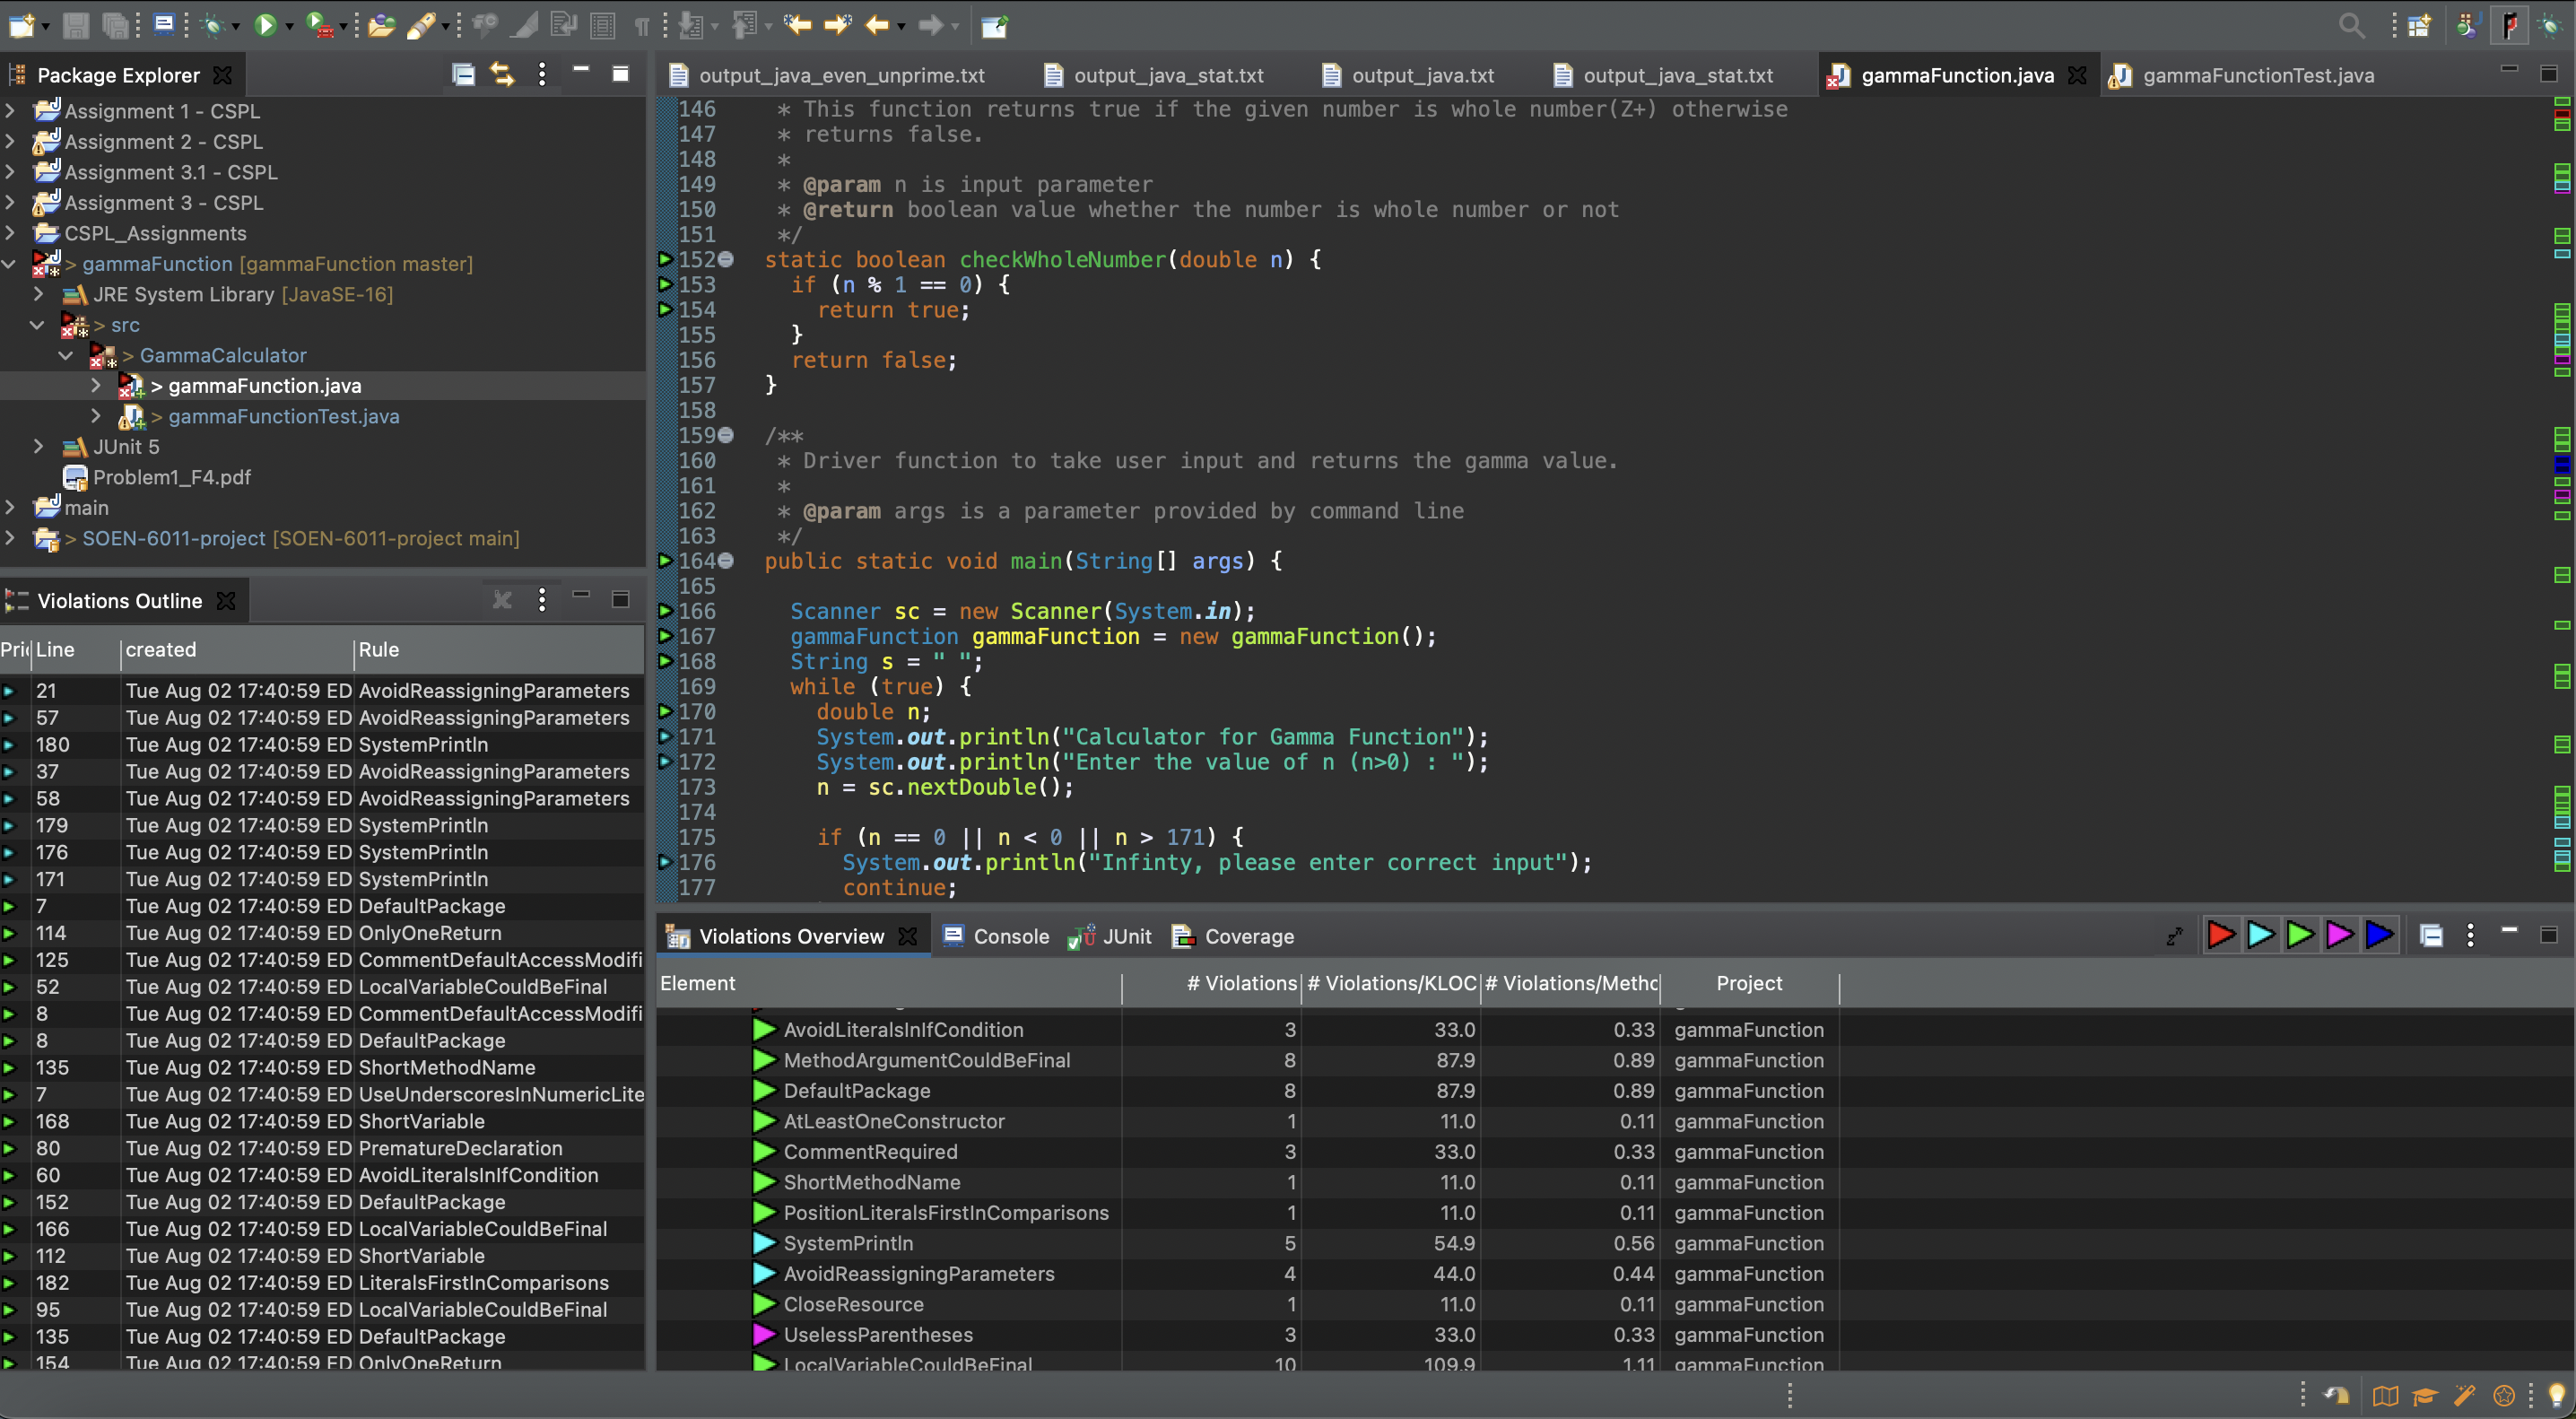
\includegraphics[width=0.9\linewidth]{Images/pmd.jpg}
    \caption{Screenshot of PMD of Gamma Function.}
    \label{fig:PMD}
\end{figure}

\subsection{Advantages}
\begin{itemize}
    \item{Several tools and editors, including Eclipse, NetBeans, IntelliJ IDEA, TextPad, Maven, Ant, and Emacs, are integrated with PMD.}
    
    \item{To detect blocks of copied and pasted code, PMD has a copy-paste detector. The best part is that the software comes with a GUI and XPath, which make it simple to write custom PMD rules.}
    
    \item{Questionable coding techniques can be highlighted by PMD, and its output is typically more pertinent and valuable.}
\end{itemize}

\subsection{Disadvantages}

\begin{itemize}
    \item{PMD has not yet published any guidelines for javadoc, comments, or indentation.}
    
    \item{Without examining the ruleset directly, it is impossible to determine which rule caused which error when running rulesets on a file or set of files.}
\end{itemize}

\newpage
\section{References}
Exception Handling in JAVA\\
\href{https://www.geeksforgeeks.org/exceptions-in-java/}{https://www.geeksforgeeks.org/exceptions-in-java/}
\\

\noindent
What is Debugging ? \\
\href{https://www.techtarget.com/searchsoftwarequality/definition/debugging}{https://www.techtarget.com/searchsoftwarequality/definition/debugging}\\

\noindent
Google CheckStyle for JAVA Programming\\
\href{https://checkstyle.sourceforge.io/google\_style.html}{https://checkstyle.sourceforge.io/google\_style.html}\\
\end{document}